%%%%%%%%%%%%%%%%%%%%%%%%%%%%%%%%%%%%%%%%%%%%%%%%%%%%%%%%%%%%%%%%%%%%%
%% This is a (brief) model paper using the achemso class
%% The document class accepts keyval options, which should include
%% the target journal and optionally the manuscript type.
%%%%%%%%%%%%%%%%%%%%%%%%%%%%%%%%%%%%%%%%%%%%%%%%%%%%%%%%%%%%%%%%%%%%%
\documentclass[journal=jacsat,manuscript=suppinfo]{achemso}

%%%%%%%%%%%%%%%%%%%%%%%%%%%%%%%%%%%%%%%%%%%%%%%%%%%%%%%%%%%%%%%%%%%%%
%% Place any additional packages needed here.  Only include packages
%% which are essential, to avoid problems later. Do NOT use any
%% packages which require e-TeX (for example etoolbox): the e-TeX
%% extensions are not currently available on the ACS conversion
%% servers.
%%%%%%%%%%%%%%%%%%%%%%%%%%%%%%%%%%%%%%%%%%%%%%%%%%%%%%%%%%%%%%%%%%%%%
\usepackage[version=3]{mhchem} % Formula subscripts using \ce{}
\usepackage[T1]{fontenc}       % Use modern font encodings

\usepackage{color}

%%%%%%%%%%%%%%%%%%%%%%%%%%%%%%%%%%%%%%%%%%%%%%%%%%%%%%%%%%%%%%%%%%%%%
%% If issues arise when submitting your manuscript, you may want to
%% un-comment the next line.  This provides information on the
%% version of every file you have used.
%%%%%%%%%%%%%%%%%%%%%%%%%%%%%%%%%%%%%%%%%%%%%%%%%%%%%%%%%%%%%%%%%%%%%
%%\listfiles

%%%%%%%%%%%%%%%%%%%%%%%%%%%%%%%%%%%%%%%%%%%%%%%%%%%%%%%%%%%%%%%%%%%%%
%% Place any additional macros here.  Please use \newcommand* where
%% possible, and avoid layout-changing macros (which are not used
%% when typesetting).
%%%%%%%%%%%%%%%%%%%%%%%%%%%%%%%%%%%%%%%%%%%%%%%%%%%%%%%%%%%%%%%%%%%%%
\newcommand*\mycommand[1]{\texttt{\emph{#1}}}

\newcommand{\cli}{Cl$^{-}$}
\newcommand{\ki}{K$^{+}$}

%%%%%%%%%%%%%%%%%%%%%%%%%%%%%%%%%%%%%%%%%%%%%%%%%%%%%%%%%%%%%%%%%%%%%
%% Meta-data block
%% ---------------
%% Each author should be given as a separate \author command.
%%
%% Corresponding authors should have an e-mail given after the author
%% name as an \email command. Phone and fax numbers can be given
%% using \phone and \fax, respectively; this information is optional.
%%
%% The affiliation of authors is given after the authors; each
%% \affiliation command applies to all preceding authors not already
%% assigned an affiliation.
%%
%% The affiliation takes an option argument for the short name.  This
%% will typically be something like "University of Somewhere".
%%
%% The \altaffiliation macro should be used for new address, etc.
%% On the other hand, \alsoaffiliation is used on a per author basis
%% when authors are associated with multiple institutions.
%%%%%%%%%%%%%%%%%%%%%%%%%%%%%%%%%%%%%%%%%%%%%%%%%%%%%%%%%%%%%%%%%%%%%
\author{T. Miteva}
\affiliation{Sorbonne Universit\'{e}s, UPMC Univ Paris 06, UMR 7614, Laboratoire de Chimie Physique Mati\`{e}re et Rayonnement, F-75005 Paris, France}

\author{N. Kryzhevoi}
\affiliation{Theoretische Chemie, Physikalisch-Chemisches Institut, Universit\"at Heidelberg, Im Neuenheimer Feld 229, D-69120 Heidelberg, Germany}

\author{N. Sisourat}
\affiliation{Sorbonne Universit\'{e}s, UPMC Univ Paris 06, UMR 7614, Laboratoire de Chimie Physique Mati\`{e}re et Rayonnement, F-75005 Paris, France}

\author{{\color{red}Kirill ?}}
\affiliation{Theoretische Chemie, Physikalisch-Chemisches Institut, Universit\"at Heidelberg, Im Neuenheimer Feld 229, D-69120 Heidelberg, Germany}

\author{{\color{red}N. Kosugi}}
\affiliation{Institute for Molecular Science, Myodaiji, Okazaki 444-8585, Japan}

\author{Ch. Nicolas}
\affiliation{Sorbonne Universit\'{e}s, UPMC Univ Paris 06, UMR 7614, Laboratoire de Chimie Physique Mati\`{e}re et Rayonnement, F-75005 Paris, France}

\author{W. Pokapanich}
\affiliation{Sorbonne Universit\'{e}s, UPMC Univ Paris 06, UMR 7614, Laboratoire de Chimie Physique Mati\`{e}re et Rayonnement, F-75005 Paris, France}

\author{Th. Saisopa}
\affiliation{Sorbonne Universit\'{e}s, UPMC Univ Paris 06, UMR 7614, Laboratoire de Chimie Physique Mati\`{e}re et Rayonnement, F-75005 Paris, France}

\author{P. Songsiriritthigul}
\affiliation{Sorbonne Universit\'{e}s, UPMC Univ Paris 06, UMR 7614, Laboratoire de Chimie Physique Mati\`{e}re et Rayonnement, F-75005 Paris, France}

\author{Y. Rattanachai}
\affiliation{Sorbonne Universit\'{e}s, UPMC Univ Paris 06, UMR 7614, Laboratoire de Chimie Physique Mati\`{e}re et Rayonnement, F-75005 Paris, France}

\author{A. Dreuw}
\affiliation{Interdisciplinary Center for Scientific Computing, Ruprecht-Karls University, Im Neuenheimer Feld 205A, D-69120 Heidelberg, Germany}

\author{J. Wenzel}
\affiliation{Interdisciplinary Center for Scientific Computing, Ruprecht-Karls University, Im Neuenheimer Feld 205A, D-69120 Heidelberg, Germany}

\author{M. Zitnik}
\affiliation{Sorbonne Universit\'{e}s, UPMC Univ Paris 06, UMR 7614, Laboratoire de Chimie Physique Mati\`{e}re et Rayonnement, F-75005 Paris, France}

\author{R. P\"{u}ttner}
\affiliation{Sorbonne Universit\'{e}s, UPMC Univ Paris 06, UMR 7614, Laboratoire de Chimie Physique Mati\`{e}re et Rayonnement, F-75005 Paris, France}

\author{J. Palaudoux}
\affiliation{Sorbonne Universit\'{e}s, UPMC Univ Paris 06, UMR 7614, Laboratoire de Chimie Physique Mati\`{e}re et Rayonnement, F-75005 Paris, France}

\author{G. \"{O}hrwall}
\affiliation{Sorbonne Universit\'{e}s, UPMC Univ Paris 06, UMR 7614, Laboratoire de Chimie Physique Mati\`{e}re et Rayonnement, F-75005 Paris, France}

\author{J.P. Rueff}
\affiliation{Sorbonne Universit\'{e}s, UPMC Univ Paris 06, UMR 7614, Laboratoire de Chimie Physique Mati\`{e}re et Rayonnement, F-75005 Paris, France}
\affiliation{Synchrotron SOLEIL, l`Orme des Merisiers, Saint-Aubin, F-91192 Gif-sur-Yvette Cedex, France}

\author{D. C\'{e}olin}
\email{denis.ceolin@synchrotron-soleil.fr}
\affiliation{Synchrotron SOLEIL, l`Orme des Merisiers, Saint-Aubin, F-91192 Gif-sur-Yvette Cedex, France}


%%%%%%%%%%%%%%%%%%%%%%%%%%%%%%%%%%%%%%%%%%%%%%%%%%%%%%%%%%%%%%%%%%%%%
%% The document title should be given as usual. Some journals require
%% a running title from the author: this should be supplied as an
%% optional argument to \title.
%%%%%%%%%%%%%%%%%%%%%%%%%%%%%%%%%%%%%%%%%%%%%%%%%%%%%%%%%%%%%%%%%%%%%
\title[]
  {RAS + XAS study of KCl aqueous solution}

%%%%%%%%%%%%%%%%%%%%%%%%%%%%%%%%%%%%%%%%%%%%%%%%%%%%%%%%%%%%%%%%%%%%%
%% Some journals require a list of abbreviations or keywords to be
%% supplied. These should be set up here, and will be printed after
%% the title and author information, if needed.
%%%%%%%%%%%%%%%%%%%%%%%%%%%%%%%%%%%%%%%%%%%%%%%%%%%%%%%%%%%%%%%%%%%%%
\abbreviations{AES,XAS}
\keywords{Solvated ions, Auger spectroscopy, X-ray absorption spectroscopy}

%%%%%%%%%%%%%%%%%%%%%%%%%%%%%%%%%%%%%%%%%%%%%%%%%%%%%%%%%%%%%%%%%%%%%
%% The manuscript does not need to include \maketitle, which is
%% executed automatically.
%%%%%%%%%%%%%%%%%%%%%%%%%%%%%%%%%%%%%%%%%%%%%%%%%%%%%%%%%%%%%%%%%%%%%
\begin{document}


\begin{figure}
\centering
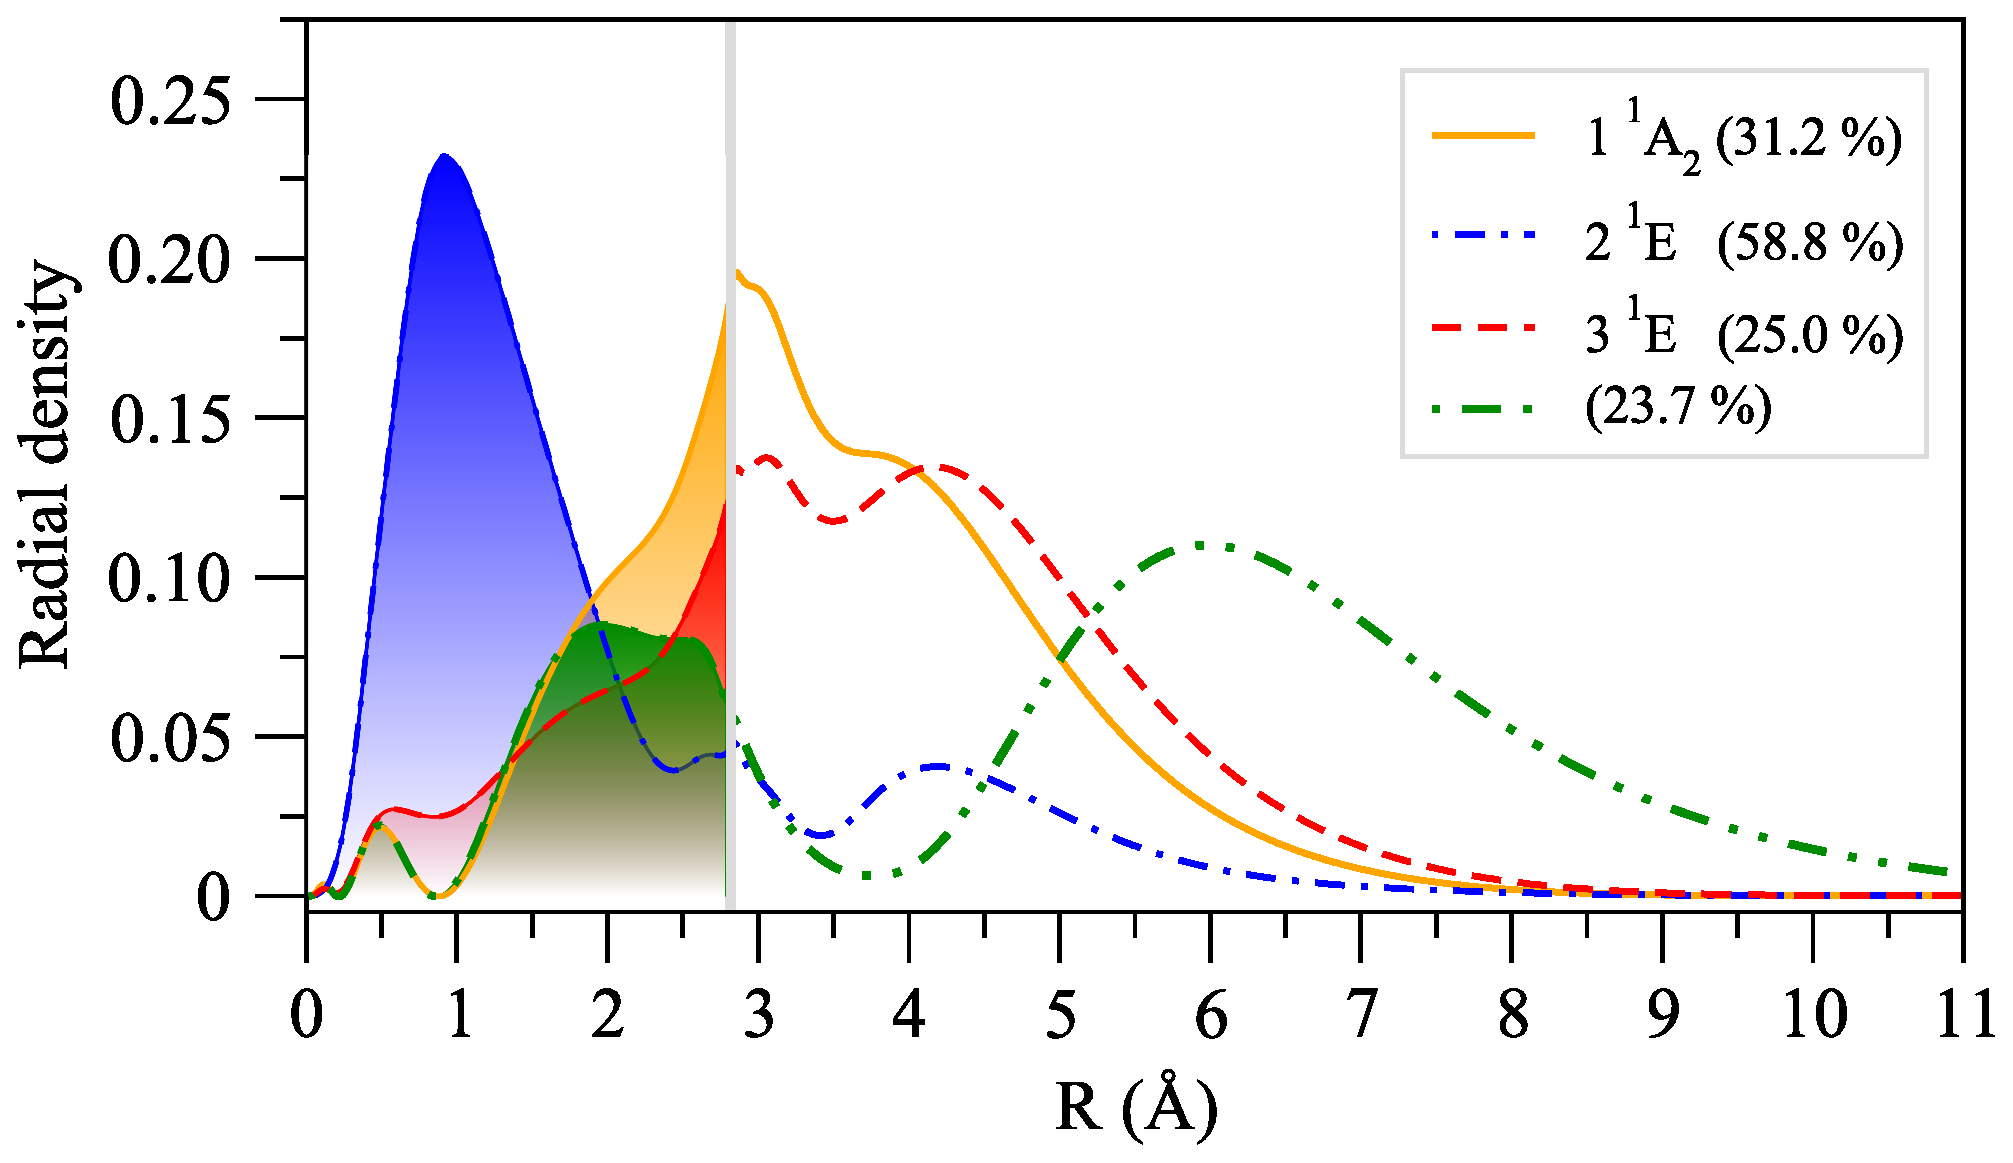
\includegraphics[scale=0.3]{figures/fg2_k_6w_okxx_55_rad_dens.eps}
\caption{Radial density distributions of the singly-occupied natural orbitals occupied by the excited electron in the core excited states 3609.11\,eV (1\,$^{1}$A$_{2}$), 3609.41\,eV (2\,$^{1}$E) and 3609.64\,eV (3\,$^{1}$E) of K$^{+}$(H$_2$O)$_6$. The grey line at 2.816\,\AA~represents the equilibrium K-O distance.}
\label{fg:rad_dens}
\end{figure}





\begin{figure}
\centering
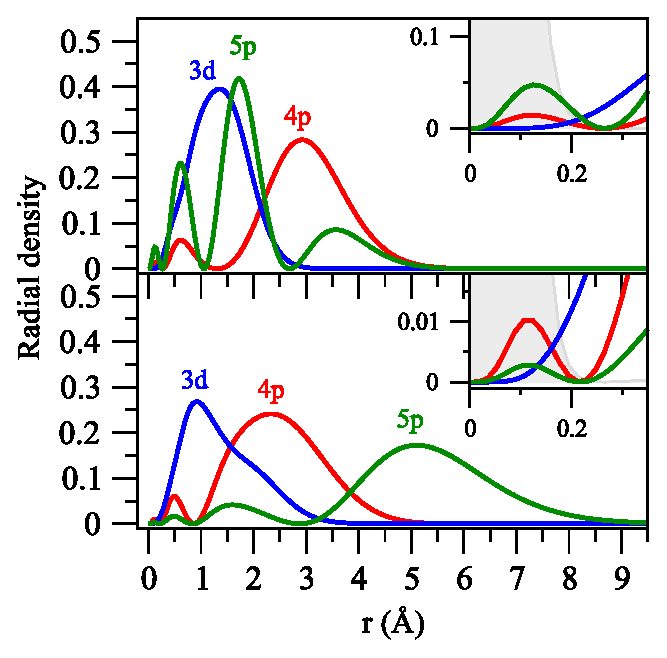
\includegraphics[scale=1.0]{figures/rad_dens_kcl.eps}
\caption{Radial density distributions of the singly-occupied natural orbital occupied by the excited electron corresponding to the 1s$\rightarrow$4p, 1s$\rightarrow$3d and 1s$\rightarrow$5p core excitations in \ki~and \cli. The insets show the region of distances relevant for the overlap with the 1s core orbital whose radial density is shown as a grey shaded area.}
\label{fg:rdens_ions}
\end{figure}

\begin{figure}
\centering
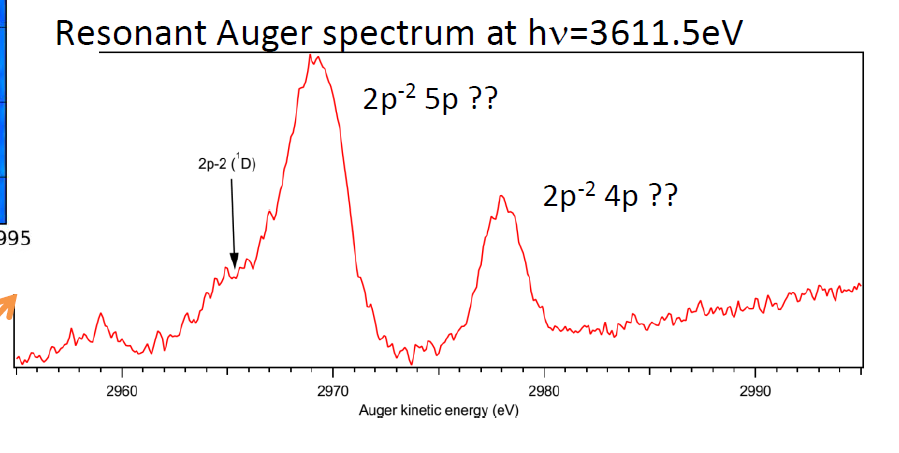
\includegraphics[scale=1.0]{figures/sfg_intensity_ratio.png}
\caption{XXX}
\label{fg:intensity_ratio}
\end{figure}




\begin{figure}[h!]
\centering
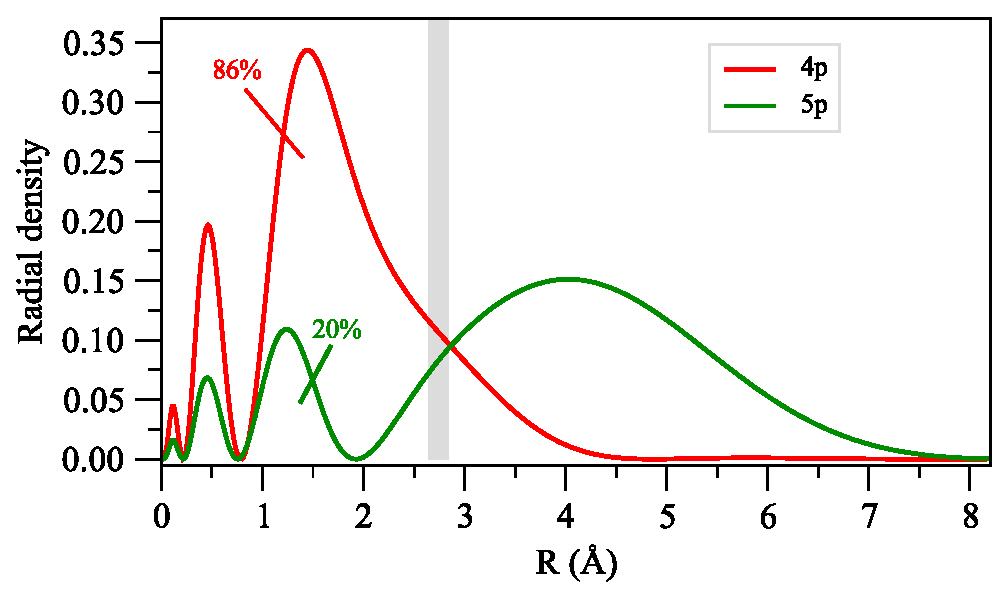
\includegraphics[scale=1.0]{figures/k_2p4_4p5p_rad_dens.eps}
\caption{Radial density distribution of the natural orbital occupied by the excited electron in the K$^{3+}$(2p$^{-2}$4p) (red) and K$^{3+}$(2p$^{-2}$5p) (green) states. The grey shaded area between 2.5\,\AA~and 3.0\,\AA~corresponds to the range of K-O distances {\color{red}in the optimized structures}.}
\label{fg:k_2p4nl_raddens}
\end{figure}


, contrary to what one would expect for a Rydberg series \citep{hussain07:022710}(MORE REF?) and contrary to what is observed for \ki. This phenomenon can be understood by the more compact radial density distribution of the excited electron in the 1s$\,\rightarrow\,$5p state compared to that of the 1s$\,\rightarrow\,$4p state shown in Fig.\ \ref{fg:rdens_ions}. As a result of this, the overlap between the core electron and the more compact 5p orbital becomes larger, and thus the oscillator strength of the transition.




\begin{table}
\begin{tabular}{c c c c}
\hline\hline
& \multicolumn{2}{c}{K$^{+}$} & K$^{+}_{\texttt{aq}}$ \\
\hline
& Ref.\ \citep{hertlein06:062715} & this work & this work \\
1s$\,\rightarrow\,$4p & 3610.7 (-8.7)& 3604.0 (-8.25 edge) & 3610.5 (Denis?)\\
1s$\,\rightarrow\,$5p & 3615.0 (-4.4) & 3608.31 (-3.94 from edge) & \\
Edge & 3619.4 & 3612.25 ($\Delta$SCF) & 3612 \\
\hline
\end{tabular}
\caption{XXX}
\end{table}



\begin{figure}
\centering
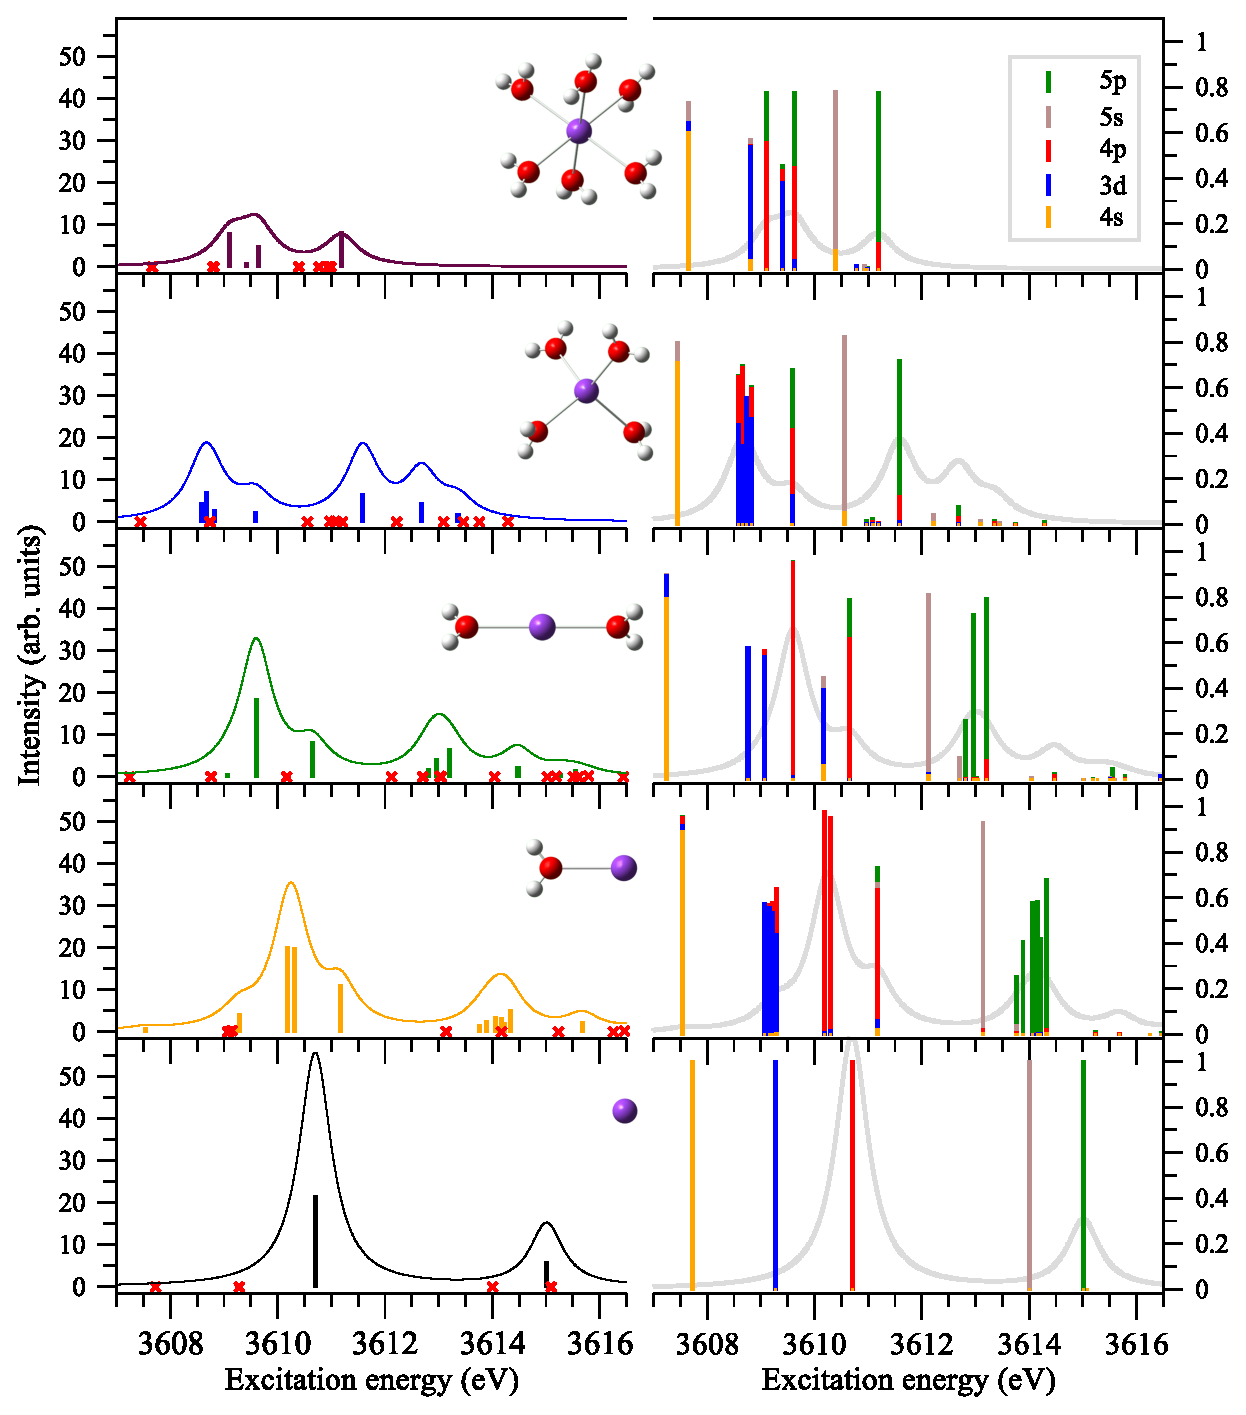
\includegraphics[scale=0.6]{figures/fg1_kh2on_xas_overlaps.eps}
\caption{Left panel: XAS spectra of the lowest core-to-valence and core-to-Rydberg transitions in the bare K$^{+}$ ion, and the microsolvated clusters K$^{+}$(H$_2$O)$_m$, $m = 1, 2, 4, 6$, computed at the CVS-ADC(2)x level of theory. The theoretical stick spectra were convolved with a Lorentzian profile of FWHM 0.74 eV in order to account for the lifetime broadening. Right panel: Projections $|a_{nl}^{i}|^2$ of the SONOs corresponding to the core excited states of the K$^{+}$(H$_2$O)$_m$ clusters with $m = 1, 2, 4, 6$ on the basis of SONOs corresponding to the 1s$\,\rightarrow\,$4s, 1s$\,\rightarrow\,$3d, 1s$\,\rightarrow\,$4p, 1s$\,\rightarrow\,$5s and 1s$\,\rightarrow\,$5p states in K$^+$ (Eq.\ \ref{eq:sono_proj}).
The theoretical X-Ray absorption spectra were shifted to higher photon energies by 6.7\,eV, which corresponds to the difference between the computed and experimental core excitation energies of the 1s $\rightarrow$ 4p excitation in the bare ion taken from Ref.\ \citep{hertlein06:062715}.}
\label{fg:knw_xas}
\end{figure}


\begin{figure}
\centering
\includegraphics[scale=0.6]{figures/clnw_xas.eps}
\caption{Left panel: XAS spectra of the lowest core-to-valence and core-to-Rydberg transitions in the bare \cli~ion, and the microsolvated clusters \cli(H$_2$O)$_m$, $m = 1, 2, 4, 6$, computed at the CVS-ADC(2)x level of theory. The theoretical stick spectra were convolved with a Lorentzian profile of FWHM 0.62 eV in order to account for the lifetime broadening (REF). Right panel: Projections $|a_{nl}^{i}|^2$ of the SONOs corresponding to the core excited states of the \cli(H$_2$O)$_m$ clusters with $m = 1, 2, 4, 6$ on the basis of SONOs corresponding to the 1s$\,\rightarrow\,$4s, 1s$\,\rightarrow\,$3d, 1s$\,\rightarrow\,$4p, 1s$\,\rightarrow\,$5s and 1s$\,\rightarrow\,$5p states in \cli~(Eq.\ \ref{eq:sono_proj}).}
\label{fg:clnw_xas}
\end{figure}


The X-ray absorption spectra of the microsolvated clusters of potassium and chlorine were computed at the ground state equilibrium geometries of K$^+$(H$_2$O)$_m$ and \cli(H$_2$O)$_m$, where m = 1, 2, 4, 6. All structures were optimized at the DFT level of theory using the B3LYP functional and the 6-311++G(2d,2p) basis set \citep{Krishnan80:650,Blaudeau97:5016}. A frequency analysis was carried out in order to confirm that the obtained geometries are minima on the respective potential energy surfaces. The geometry optimization and frequency analysis were performed with the Gaussian 09 package \citep{g09}. In the case of K$^{+}$(H$_2$O)$_6$ the ground state geometry was obtained by constrained geometry optimization starting with the equilibrium geometry \citep{lee99:3995} belonging to the D$_3$ point group and increasing the angle $\theta$ between the K-O bond and the $C_3$ axis to 55$^{\circ}$. This angle was chosen to be around the maximum in the O-K-O angular distribution obtained from quantum mechanics / molecular mechanics dynamical simulations in Ref.\ \citep{ma14:1006}. {\color{red} the maximum is at 70$^{\circ}$, in our calculation the angle is 90$^{\circ}$} The ground state equilibrium structures are presented in Fig.\ \ref{fg:xas_kcl}. In the case of potassium, they belong to the C$_{2\text{v}}$ (K$^{+}$(H$_2$O)), D$_{2\text{d}}$ (K$^{+}$(H$_2$O)$_2$), S$_4$ (K$^{+}$(H$_2$O)$_4$), and D$_3$ (K$^{+}$(H$_2$O)$_6$) point groups \citep{rao08:12944}. The optimized K-O distances are between 2.638 -- 2.842~\AA, which is in good agreement with other theoretical and experimental works \citep{Ohtaki93:1157,soper06:180,ma14:1006}. In the case of chlorine, the ground state equilibrium 1-, 2- and 6-coordinated structures belong to the C$_{1}$ point group, whereas the 4-coordinated structure belongs to the C$_4$ point group \citep{gora00:7}. The optimized Cl-O distances are between 3.093 -- {\color{red}3.305}~\AA, which is in good agreement with other theoretical and experimental works \citep{ge13:13169,gora00:7,Ohtaki93:1157,soper06:180,ma14:1006}. The 6-coordinated clusters can be considered as representatives of the complete first solvation shell of the two ions \citep{Ohtaki93:1157,soper06:180,ma14:1006}.


The energies and transition moments of the core excited states of the microsolvated clusters were computed with the algebraic diagrammatic construction method for the polarization propagator \citep{sch82:2395} within the core-valence separation approximation \citep{bar85:867,ced80:206,ced81:1038} (CVS-ADC(2)x) as implemented in the Q-Chem package \citep{Wenzel14:1900,Wenzel14:4583,Wormit14:774,QChem2015}. In the case of \cli, the 6-311++G(3df,3pd) basis set \citep{Krishnan80:650,McLean80:5639} (excluding the f functions) was used on all atoms, whereas in the case of \ki, we used the 6-311+G(2d,p) basis set \citep{Krishnan80:650,Blaudeau97:5016} on all atoms, and an additional set of 2s, 2p and 2d diffuse functions was added on K. In our calculations, the core space comprises the 1s orbital of K$^{+}$ or \cli, whereas the remaining occupied orbitals are included in the valence space. For the calculations of the XAS spectra we used the D$_2$ point group in the case of K$^{+}$(H$_2$O)$_2$, the C$_2$ point group in the case of K$^{+}$(H$_2$O)$_4$, K$^{+}$(H$_2$O)$_6$ and \cli(H$_2$O)$_4$. To account for the experimental resolution and for the lifetime broadening due to the Auger decay of the core excited states, we convolved the theoretical spectra with a {\color{red} (Denis, exp. resolution? ) Voigt profile with a Gaussian of FWHM XX\,eV} and a Lorentzian of FWHM 0.74\,eV and 0.62\,eV in the case of \ki~and \cli, respectively \citep{Krause79:329}. We analyzed the core excited states by expanding the singly occupied natural orbitals (SONOs) $\psi_{i}$ of the microsolvated clusters in the basis of SONOs of the bare K$^{+}$ or \cli~ion $\chi_{nl}$
%
\begin{equation}\label{eq:sono_proj}
\psi_{i} = \sum_{nl} a^{i}_{nl} \chi_{nl}
\end{equation}
%
where $n$ and $l$ stand for the principal and orbital quantum numbers as described in Ref.\ \citep{miteva16:16671}. The expansion coefficients $a^{i}_{nl}$ show the degree of delocalization of the excited electron and the mixing of the core excited states in the crystal field created by the surrounding water molecules (see Fig.\ \ref{fg:xas_kcl}).


The final states following KLL resonant Auger decay of K$^{+}$ and \cli~were computed at the Configuration Interaction Singles (CIS) level using the Graphical Unitary Group Approach (GUGA) as implemented in the GAMESS-US package \citep{GUGA_PhysScr_21,GUGA_JCP_70,GUS}. We used the 6-311++G(2d,2p) basis set \citep{Blaudeau97:5016} augmented with 2s, 2p, 2d diffuse functions on \ki, and the cc-pVTZ basis set augmented with 6s, 6p, 6d diffuse KBJ functions \citep{Kaufmann89:2223} on \cli. The active space comprises the 2s and 2p orbitals of K/Cl with occupancy fixed to 6 and all virtual orbitals with occupancy fixed to 1. The remaining doubly occupied orbitals were frozen in the calculation. \citep{mosnier16:061401}



%%%%%%%%%%%%%%%%%%%%%%%%%%%%%%%%%%%%%%%%%%%%%%%%%%%%%%%%%%%%%%%%%%%%%
%% The appropriate \bibliography command should be placed here.
%% Notice that the class file automatically sets \bibliographystyle
%% and also names the section correctly.
%%%%%%%%%%%%%%%%%%%%%%%%%%%%%%%%%%%%%%%%%%%%%%%%%%%%%%%%%%%%%%%%%%%%%
%\bibliography{F:/Articles/biblography/Bibliography}

\end{document}
